%%Section4-5

\section{実験装置}
\begin{figure}[h]
  \begin{center}
    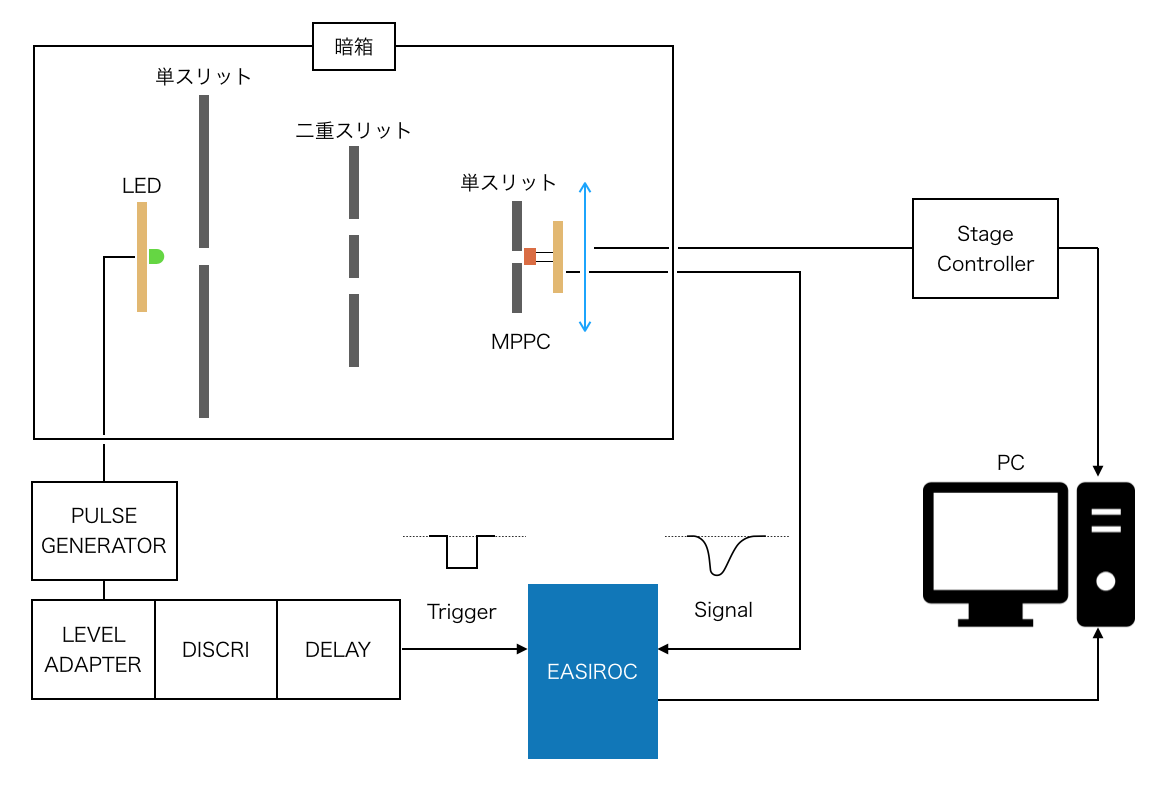
\includegraphics[width=12cm]{setup2019.png}
  \end{center}
  \caption{実験の模式図}
\end{figure}

本実験で用いる実験装置。
\begin{itemize}
  \item 光源(LED)
  \item 光検出器(MPPC)
  \item MPPC読み出しモジュール(EASIROC)
  \item スリット(単スリット・二重スリット)
  \item 可動式ステージ\par
        「Stage Controller」で制御。MPPCが設置されている基盤の位置を可動式ステージで細かく変更することが可能。
  \item 波高発生器(PULSE GENERATOR)\par
        非常に高い(1kHz)周期で矩形波を出力。出力と同期してトリガーを出力することも可能。
  \item レベルアダプター(LEVEL ADAOTER)\par
        TTL 入力信号をNIM 信号に変換し、出力。
  \item ディスクリミネータ(DISCRIMINATOR)\par
        アナログ入力信号の大きさがあるしきい値以上の場合に論理信号を出力。
  \item 遅延回路(DELAY)\par
        信号を遅らせるもの。要は長いケーブル。
  \item 測定用PC \par
        EASIROCの制御や、可動式ステージの制御を行う。データ取得まで行うことができる。
\end{itemize}
光学機器を図のように並べ、光の干渉を起こす。各デバイスの位置や距離によって干渉の見え方が変わるが、これは実際に物を置いていろいろ試してみるとよい。以下では、光検出器とその読み出しについて説明する。

\subsection{MPPC}
MPPC(Micro Pixel Photon Counter)はAvalamche Photo Diode(APD)が多数配列された光検出器である。APDは半導体でできている。P型とN型、異なるドープ型の半導体にある向きで電圧をかけると、キャリアの少ない空乏層ができる。ここに光子が入射すると、光電効果で電子をはじき出す。電子は印加電圧によってエネルギーを持ち、さらに周囲の原子殻内電子をはじき出し、雪崩(Avalanche)的に電子を倍増する。印加電圧によって様々な倍増モードがあるが、MPPC内のAPDでは、十分な印加電圧をかけることで入射光子数によらない出力電流を得る(ガイガーモード)。このガイガーモードAPDが多数配列することにより、我々は光子が入射したAPDのチャンネル数だけを数えることで、(pile upはあるものの)光子数をデジタルに数えることができる。
\begin{figure}[h]
  \begin{tabular}{ccc}
    \begin{minipage}[t]{0.33\hsize}
      \begin{center}
        \includegraphics[width=4cm]{mppc.jpg}
      \end{center}
      \caption{MPPC}
    \end{minipage}
    \begin{minipage}[t]{0.33\hsize}
      \begin{center}
        \includegraphics[width=4cm]{APDstructure.PNG}
      \end{center}
      \caption{APD}
    \end{minipage}
    \begin{minipage}[t]{0.33\hsize}
      \begin{center}
        \includegraphics[width=4cm]{QuenchingArray.PNG}
      \end{center}
      \caption{MPPCはAPDを並列に並べたもの}
    \end{minipage}
  \end{tabular}
\end{figure}
浜松ホトニクスのハンドブックに、詳細なMPPCの挙動が説明されている。\cite{hamamatsu}
\subsection{EASIROC}
EASIROCモジュールは、書き換え不可能な集積回路(ASIC)であるEASIROCチップと、EASIROCチップ制御用の書き換え可能な集積回路(FPGA)であるArtix7が搭載された、MPPCの(多チャンネネル)読み出しモジュールである。今回は1チャンネルしか使わないし、FPGAのfirmwareの書き換えも(おそらく)ないので、ここでは、EASIROCチップの回路の概要と、アナログな出力波形について見ることにする。\\
EASIROCチップは、Pre-Amp,Shaper,Discriminator,Capacitorからなる。Pre-Amp,Slow Shaperを通った信号電圧をCapacitorに保存し、Trigger信号が入力されたときに電圧をholdし、ADC(Analog Digital Converter)でデジタル情報に変換する。
\begin{figure}[h]
  \begin{center}
    \includegraphics[width=12cm]{EASIROCCircuitDiagram.PNG}
  \end{center}
  \caption{EASIROC回路概略}
\end{figure}

\begin{figure}[h]
  \begin{tabular}{cccc}
    \begin{minipage}[t]{0.25\hsize}
      \begin{center}
        \includegraphics[width=4cm]{preamp.BMP}
      \end{center}
      \caption{Pre-Amp}
    \end{minipage}
    \begin{minipage}[t]{0.25\hsize}
      \begin{center}
        \includegraphics[width=4cm]{fastshaper.BMP}
      \end{center}
      \caption{Fast Shaper}
    \end{minipage}
    \begin{minipage}[t]{0.25\hsize}
      \begin{center}
        \includegraphics[width=4cm]{slowshaper.BMP}
      \end{center}
      \caption{Slow Shaper}
    \end{minipage}
    \begin{minipage}[t]{0.25\hsize}
      \begin{center}
        \includegraphics[width=4cm]{slowshaperhold.BMP}
      \end{center}
      \caption{holdしたSlow Shaper}
    \end{minipage}
  \end{tabular}
\end{figure}


各デバイスを通った信号の出力波形は、EASIROCモジュールのProbe出力を観察するとわかる。Fast ShaperはSelf Trigger用なので、今回は(おそらく)使わない。Trigger信号に合わせてShaperの波高の一番高いところが読み出されているのがわかる。Trigger信号とShaperの立ち上がりがきちんと合うかどうかはケーブルの長さやDelayモジュールによって操作できる。

\section{測定方法}

\subsection{可動式ステージの使用方法}

可動式ステージは、stage.pyを用いて制御する。使用するためのコマンドは、以下の通りである。
\begin{lstlisting}[caption=stage.pyのコマンド]
\$ python stage.py [コマンド]  
\end{lstlisting}

\begin{table}[htbp]
  \begin{center}
    \caption{stage.py コマンド一覧}
    \begin{tabular}{|l|l|l|} \hline
      入力コマンド & 使い方       & 動作                                      \\ \hline \hline
      -o           & -o           & left or right 側の原点に戻る              \\ \hline
      -r           & -r           & データリセット、現在地を原点とする        \\ \hline
      -mr          & -mr [整数値] & 今いるところから[整数値]パルス分+側へ移動 \\ \hline
      -ml          & -ml [整数値] & 今いるところから[整数値]パルス分-側へ移動 \\ \hline
      -pr          & -pr [整数値] & 絶対的な座標位置+[整数値]パルスへ移動     \\ \hline
      -pl          & -pl [整数値] & 絶対的な座標位置-[整数値]パルスへ移動     \\ \hline
      -s           & -s           & 動作停止                                  \\ \hline
      -q           & -q           & ステージの情報を表示                      \\ \hline
      -h           & -h           & コマンドの使い方表示                      \\ \hline
    \end{tabular}
  \end{center}
\end{table}

\begin{itembox}[l]{注意事項}
  \begin{itemize}
    \item 動く距離とパルスの関係は2μm/パルス。
    \item 一度の操作で送ることのできるコマンドは1つ。
    \item 複数送った場合、コマンド一覧の上から順に優先順位がついており、優先順位が最も高いものの動作を行う。
  \end{itemize}
  例えば、{\tt \$ ./stage.py -ml 1000 -mr 20000 -s -o +} とコマンドを送っても, {\tt -o} のみが認識される。
\end{itembox}


\subsection{EASOROCの使用方法}

\subsubsection{EASIROCモジュールへのアクセス}

\begin{lstlisting}[caption=EASIROCモジュールへのアクセス]
  \$ EASIROC/easiroc/easiroc 192.168.10.102 3
\end{lstlisting}
でEASIROCモジュールへのアクセスが可能になる。数字の部分はEASIROCのIPアドレス。

\begin{lstlisting}
\$ cd EASIROC/easiroc
\$ ./easiroc 192.168.10.102 3

\ I'm : 192.168.10.102
\ Please select
\ 1. Transmit SC
\ 2. Tranmit Read SC
\ 3. ASIC Initialize
\ 4. Transmit Probe
\ 5. Connection Close
\ 6. Start DAQ
\ 7. Debug
\ input # === >
\end{lstlisting}
{\tt ”Please select''} 以降の文字が表示されていればOK。以降でこれら7つのコマンドを使い分け、EASIROCを操作する。主な各コマンドの操作内容は次のようになっている。

\begin{table}[htbp]
  \begin{center}
    \caption{easiroc コマンド一覧}
    \begin{tabular}{|l|l|} \hline
      入力コマンド & 動作                                                     \\ \hline \hline
      1            & EASIROC 測定後でもオシロスコープで波形を見ることができる \\ \hline
      2            & どのチャンネルを出力するかを決める                       \\ \hline
      5            & 接続を切る                                               \\ \hline
      6            & 測定開始                                                 \\ \hline
    \end{tabular}
  \end{center}
\end{table}

今回はch.12から出力される信号のみを見るため、コマンド"2"の出番はない。

\subsubsection{印加電圧の設定}

EASIROC起動後に
\begin{lstlisting}[caption=印加電圧の設定]
  \$ cd EASIROC/easiroc/easiroc_UDPcontrol
  \$ ./udp102
\end{lstlisting}
を実行することで、印加電圧を設定することができる。udp102を実行する。(102はIPアドレスの最後のところ)
\begin{table}[htbp]
  \begin{center}
    \caption{UDPcontrol コマンド一覧}
    \begin{tabular}{|l|l|} \hline
      入力コマンド & 動作                                                            \\ \hline \hline
      1            & HighVoltageの設定(この時打った電圧が全チャンネルに反映される) \\ \hline
      2            & HighVoltageのステータス                                         \\ \hline
      3            & 実際にかかっている電圧                                          \\ \hline
      5            & exit                                                            \\ \hline
    \end{tabular}
  \end{center}
\end{table}

\begin{itembox}[l]{注意事項}
  \begin{itemize}
    \item easirocで接続してからudp102を起動
    \item 電流は正常な値で数uA 程度である。10 倍以上の電流が流れるようであればすぐにHighVoltage を0 にすること
    \item udp102を終了してからeasirocの接続を切る\par
          (切るときはHighVolの設定を0にしてから何度か2でステータスを確認して、4V程度になったことを確認してから切る)
    \item 1で電圧をかける前に変な電圧がかかっていないか2でステータスを確認する
  \end{itemize}
\end{itembox}

\subsubsection{EASIROC測定手順}

2つの実行ファイルを並行して操作する必要があるため、2つのウィンドウを立ち上げる。これらを今後、ウィンドウ1,ウィンドウ2と区別する。また、測定結果も測定時に同時に確認したい場合は、ウィンドウを3つ用意する。

\begin{enumerate}
  \item EASIROCモジュールへアクセスする(ウィンドウ1)
  \item 印加電圧を設定する(ウィンドウ2)
  \item ウィンドウ2でコマンド''2''を打って印加電圧を設定する。印加電圧は53.5から54V程度が好ましく、それ以上に設定するとMPPCに負担がかかるため極力上げないこと。
  \item ウィンドウ1でコマンド''1''→''2''を入力し、オシロスコープにて波形を確認する。
  \item ウィンドウ1でコマンド''6''を入力し、測定を開始する\par
        \begin{lstlisting}[caption=測定手順]
\ input # ===>6
\ Input output data file name : ファイル名.dat
\ Input total # of events =====> 欲しいイベント数
\end{lstlisting}
  \item 測定結果の確認\par
        別ウィンドウ(ウィンドウ3)にて、
        \begin{lstlisting}[caption=測定結果の確認]
\$ root
\ root[0] .L fullcheck6.C
\ root[1] fullcheck6(''ファイル名.dat'')
\ root[2] TBrowser tb
\end{lstlisting}
        TBrowserが起動するので,その中から{\tt ファイル名.root}を探してその中のch.12に保存されているプロットが測定結果。
\end{enumerate}
rootの使い方に関しては、6.4節を参照。\par
データの収集方法についても、詳しくはマニュアル参照。EASROCボードのそれぞれのチャンネルが何をするものかは、User Guideの1章を参照すること。2章には、EASIROCボードの制御法が記されている。User Guideに簡単な操作法が記されているが、ボード仕様書にはさらに細かい情報が載っているので、困ったら参照すること。
